\documentclass[journal]{IEEEtran}
\usepackage{graphicx} % Required for inserting images
\usepackage{array}
\usepackage{booktabs}
\usepackage{amsmath}
\usepackage{float}
\usepackage{url}
\title{Decoding Tai Phake Through Vision:\\ Introducing TP-VSD11 for Visual Speech Recognition}
\author{
Milinda Barua\textsuperscript{1},
Gargi Hatibaruah\textsuperscript{2},
Ishani Phukan\textsuperscript{3}\\
Champak Handique\textsuperscript{4},
Dhiraj Kalita\textsuperscript{5},
Rabinder Kumar Prasad\textsuperscript{6}\\[0.3cm]
\textit{Department of Computer Science and Engineering}\\
\textit{Dibrugarh University}\\
Dibrugarh, Assam, India\\[0.2cm]
\textsuperscript{1}milindabarua04@gmail.com,
\textsuperscript{2}gargihbaruah@gmail.com,
\textsuperscript{3}ishani.phukan04@gmail.com,
\textsuperscript{4}champak272004@gmail.com,
\textsuperscript{5}rs\_dhirajkalita@dibru.ac.in,
\textsuperscript{6}rkp@dibru.ac.in
\vspace{-8pt}
}
\date{\today}
\raggedbottom
\begin{document}
\maketitle
\begin{abstract}
    Visual Speech Recognition (VSR) identifies speech from lip movements without audio. Developing VSR for low-resource languages remains difficult due to very less digital resources and datasets. This study focuses on VSR for Tai Phake, an endangered language of Assam spoken by approximately 2,000 people worldwide. We have compared three architectures: EfficientNetB0-BiLSTM, EfficientNetB0-BiGRU, and EfficientNetB0-Lightweight Transformer. Using the custom digit dataset, TP-VSD11 (Tai Phake Visual Speech Dataset for 11 digits), and speaker-independent 5-fold GroupKFold evaluation, BiLSTM achieves 90.45\% accuracy, outperforming BiGRU (87.18\%) and Transformer (86.82\%). Error analysis reveals misclassifications associated with similar visual mouth movements and phonemic similarities, highlighting the importance of data verification in low-resource speech technologies. A non-temporal baseline achieves 74.5\%, demonstrating the contribution of temporal sequence modelling to Tai Phake visual speech recognition.

    \textbf{Keywords}: Visual Speech Recognition, Low Resource Language, Tai Phake, EfficientNetB0, Bidirectional Long Short-Term Memory (BiLSTM), Bidirectional Gated Recurrent Unit (BiGRU), Transformer, Digit Recognition
\end{abstract}


\section{Introduction}
Visual Speech Recognition (VSR), or lip-reading, recognizes speech by analysing lip and mouth movements across video frames without audio. It is useful when audio is unavailable or unclear \cite{fernandezlopez2018survey}. Deep learning has improved VSR by learning spatial and temporal patterns from video. The Lip Reading in the Wild (LRW) dataset contains 500 English word classes collected from BBC programmes \cite{chung2016lipreading}, while Lip Reading Sentences in the Wild focuses on complete phrases and sentences \cite{chung2017sentences}. However, VSR development for low-resource languages remains challenging due to very less labelled video data and digital resources \cite{magueresse2020low}, making language-specific datasets a necessity.

India has considerable linguistic diversity, with 22 Scheduled and 99 Non-Scheduled Languages reported in the 2011 Census \cite{census2011language}. Research on visual speech recognition (VSR) has covered several Indian languages, including Hindi, Kannada, Marathi, Assamese, and Khasi. For Hindi, \cite{patil2019hindi} explored lip reading with an LSTM model and mouth-related features while \cite{rudregowda2023kannada} used a VGG16-based CNN for Kannada. In the case of Marathi, \cite{kulkarni2024marathi} introduced a lip-reading dataset and tested different neural network approaches. \cite{prasad2025analysis} investigated Assamese digit recognition using a custom video dataset and CNN-LSTM model, whereas \cite{lyngdoh2026khasi} studied Khasi digit lip-reading (zero to nine) using videos from nine speakers, MediaPipe-based lip extraction, and machine learning classifiers. These studies demonstrate the potential of language-specific VSR, although their tasks and methodologies differ.

Assam is home to several linguistic communities, including Assamese, Bodo, Mising, and Tai-speaking groups. The Tai-Ahoms migrated to present-day Assam in the thirteenth century under Siu-kha-pha and ruled for approximately 600 years, until the nineteenth century. The Tai Phake community migrated from the Hu-Kwang Valley to Assam around 1775 in search of a better life \cite{lahkar2019origin}. Also known as Phakial, Tai Phake is spoken by an estimated 2,000 people worldwide, according to the Scheme for Protection and Preservation of Endangered Languages \cite{deka2025studying}. Its speakers mainly reside in the Dibrugarh and Tinsukia districts \cite{sppeletaiphake}. Morey  documented Tai Phake and other Tai languages of Assam, covering their grammar, sound systems, vocabulary, and writing systems\cite{morey2005tailanguages}.

Tai Phake has six lexical tones, distinct vowel sounds, and variations in vowel length \cite{morey2020syllable}. However, VSR relies only on visible mouth movements rather than  acoustic information. Lexical tones are mainly dependent on pitch changes and vibrations of the vocal fold. These features are difficult to observe through lip movements alone. In our study, the 11 digit classes ($d_0$ to $d_{10}$) are mainly distinguished by their consonants and vowels rather than tone. No tonal minimal pairs are present among these classes. Therefore, the model focuses on visible mouth movements, such as closing both lips, touching the tongue to the teeth, and rounding the lips. Acoustic information about tone is not required for this visual recognition task. Our search found no published VSR system or visual speech dataset for Tai Phake. Therefore, we created the TP-VSD11 data set. It consists of 1,100 video samples from 100 native speakers across 11 classes ($d_0$ to $d_{10}$). Using a speaker independent split, we developed a Tai Phake digit recognition system to evaluate its ability to recognize digits spoken by previously unseen speakers. We used Dlib facial landmarks to locate the mouth and resized the images to $128 \times 128$ pixels. We tested three models: EfficientNetB0-BiLSTM, EfficientNetB0-BiGRU, and EfficientNetB0-Lightweight Transformer. The system uses only visual information and does not require audio. To maintain speaker independence, five-fold (GroupKFold) cross-validation was used. Each fold consisted of a training set of 80 speakers and a test set of 20 unseen speakers. The data were split into their own speaker groups, ensuring speaker independence. In this paper, a baseline was established for experimentation on Tai Phake digit recognition. Three models were compared, and the factors affecting recognition were analysed. The dataset created (TP-VSD11) and results obtained can be used to aid future work on VSR within Tai Phake and other low resource languages of Northeast India. The methodology can be found in Section~\ref{sec3}.

\section{Related Work} \label{sec2}

A vast amount of work has been undertaken to study VSR. Early work focused on the study of English using various datasets and networks, but recent studies have focused on multi-language and low-resource languages. This section looks at various international and Indian works that have been undertaken in the field of Visual Speech Recognition. A review is provided into various datasets and methods for lip reading.
\subsection{\textit{International Research}}

Chung and Zisserman \cite{chung2016lipreading} introduced the Lip Reading in the Wild (LRW) dataset, containing 500 English word classes collected from BBC television programmes. Later, \cite{chung2017sentences} introduced the Lip Reading Sentences in the Wild (LRS) dataset. It was designed to recognize full phrases and sentences from videos. These datasets helped researchers develop and test VSR systems. To study lip reading across various languages, \cite{ma2022multilingualvsr} explored multilingual VSR. Their study showed that model design, training data, data augmentation, and other learning tasks can affect recognition results. They also found that using data from other languages can help when there is limited data for the target language.
\cite{kim2023lowresource} studied lip reading for languages with limited video data. They used knowledge from languages with more data to help recognize languages with less data. They tested their method on English, Spanish, French, Italian, and Portuguese. Their results showed that knowledge from other languages can help when training data are limited.
Researchers have also developed datasets for underrepresented languages. \cite{rahmatullah2024idlr} introduced the Indonesian Lip Reading (ID-LR) dataset, containing 105,300 videos across 230 word classes. For Persian, \cite{peymanfard2024armanav} introduced the Arman-AV dataset, containing approximately 220 hours of recordings from 1,760 speakers. Their study also examined visemes, which represent speech sounds with similar visible mouth movements. Unlike this audio-visual dataset, the present study uses only visual information.

These studies demonstrate the importance of language-specific datasets, suitable temporal models, and speaker diversity in VSR. They also highlight the challenges of developing reliable recognition systems when large video datasets are unavailable.

\subsection{\textit{National Research}}

In India, VSR research has covered Hindi, Kannada, Marathi, Indian English, Assamese, and Khasi. For Hindi, \cite{patil2019hindi} developed an LSTM-based lip-reading system using geometric mouth features and recordings from 50 speakers to recognize words and sentences. Their study also showed that sentence recognition is more challenging than recognizing a smaller set of words. For Kannada, \cite{rudregowda2023kannada} used a VGG16-based CNN for lip reading. \cite{kulkarni2024marathi} created a Marathi lip-reading dataset and tested different neural networks.

For Indian English, \cite{indian2024audiovisual} created a dataset using Dlib to extract mouth regions and an LSTM model for recognition. Their study compared audio-based, visual-only, and audio-visual recognition, with the visual-only approach being particularly relevant to the present work. Similarly, \cite{lipbengal2025} presented LipBengal, a dataset of 150 speakers covering 54 Bengali classes, including phonemes, alphabets, and symbols. In Assam, \cite{prasad2025analysis} studied Assamese digit lip-reading using a custom video dataset and different deep learning models. Their CNN-LSTM model achieved 83\% accuracy. Similarly, \cite{lyngdoh2026khasi} studied Khasi digit lip-reading using videos from nine speakers across ten classes (zero to nine). They extracted lip features using MediaPipe and applied PCA with Support Vector Machine (SVM) and K-Nearest Neighbors (KNN), achieving test accuracies of 94.44\% and 80.86\%, respectively. Although this study is relevant to digit recognition in Northeast India, direct accuracy comparisons are not appropriate because the datasets and evaluation protocols differ.

Overall, Indian studies demonstrate the use of different datasets, features and learning architectures can be used for language specific lip reading tasks. However, the recognition task and size of data has varied. Through literature searching it was found there was no published VSR system, or visual speech data set for Tai Phake. This indicates there is a need for more work. This study provides a visual only data set of 11 classes (from $d_0$ to $d_{10}$) of digits spoken by 100 speakers known as TP-VSD11. Features were extracted from the mouths of each video frame and used to train three deep learning architectures. The data has been separated into speaker independent partitions, meaning the validation speakers were not included in the training data. This study uses visual information only, unlike audio based and audio-visual systems, to provide an initial baseline for the recognition of digits in Tai Phake. This helps understand the recognition challenges. The method can be seen in Section~\ref{sec3}.

\section{Methodology} \label{sec3}
In this work, we have included three models: EfficientNetB0-BiLSTM, EfficientNetB0-BiGRU and EfficientNetB0 Transformer. Then we compared the accuracies we got after training and testing these models. The proposed architectures are illustrated in Fig. \ref{fig:architecture_diagram}.
\begin{figure}[!t]
    \centering
    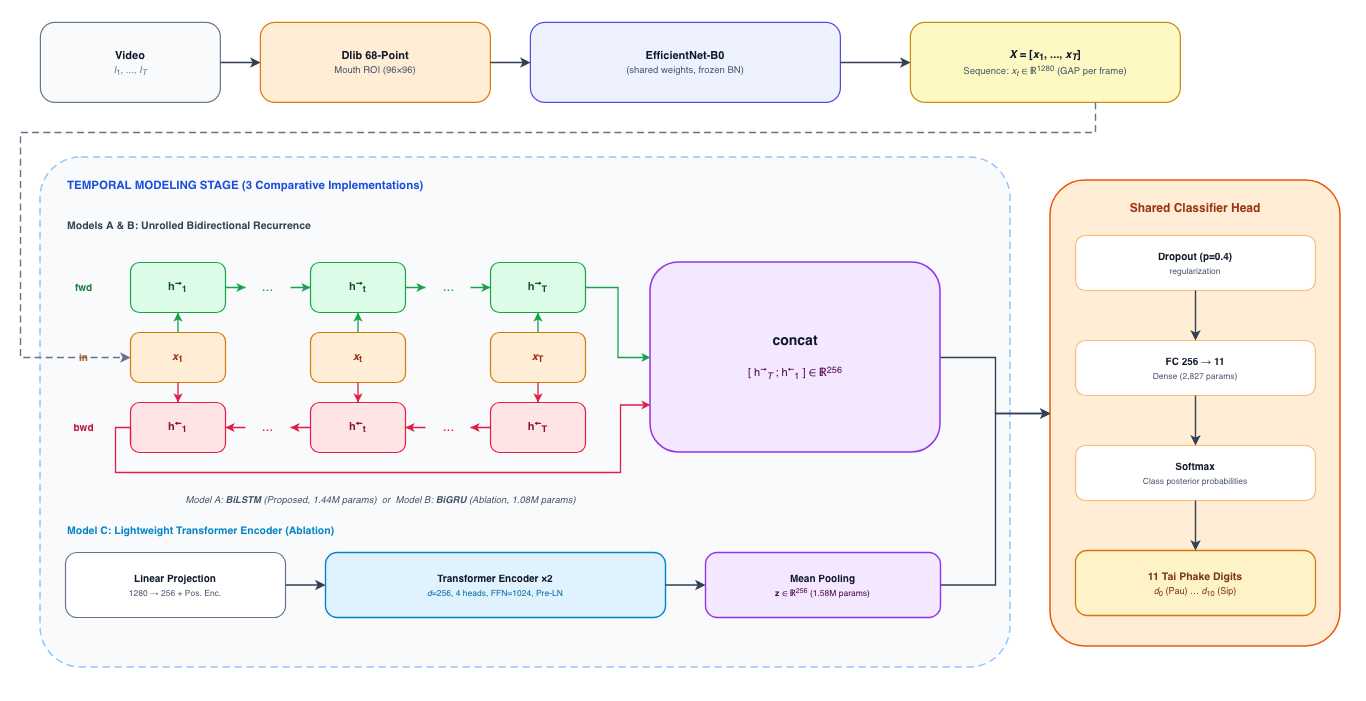
\includegraphics[width=1.0\linewidth]{architecture_combined.drawio.png}
    \caption{Comparative architectures for Tai Phake visual speech recognition, sharing an identical EfficientNetB0 spatial front-end with three distinct temporal modules.}
    \label{fig:architecture_diagram}
\end{figure}

\subsection{Dataset Collection and Preprocessing}

The Tai Phake Visual Speech Digit dataset, TP-VSD11, contains 1,100 video samples collected from 100 speakers (50 male and 50 female), covering 11 digit classes from 0 (Pao) to 10 (Sip). Collecting data was particularly challenging because of the very small number of Tai Phake speakers worldwide, making dataset development a major contribution of this study. Each speaker recorded the digits using a phone camera at 30 frames per second (FPS), with videos stored in MP4 format at a resolution of $1280 \times 720$ pixels. Each video shows one digit. Videos are stored in speaker folders and named `d{clipIndex}.mp4` for easy identification and testing.

All videos were recorded indoors with good lighting, a plain background, and a camera placed at eye level, 0.5 meters from the speaker. Participants were asked to say the digits naturally. Two native Tai Phake speakers checked the video labels and achieved a Cohen's $\kappa$ score of 0.93 .All 100 participants agreed to take part in the study for research and language preservation.
\begin{figure}[htbp]
    \centering
    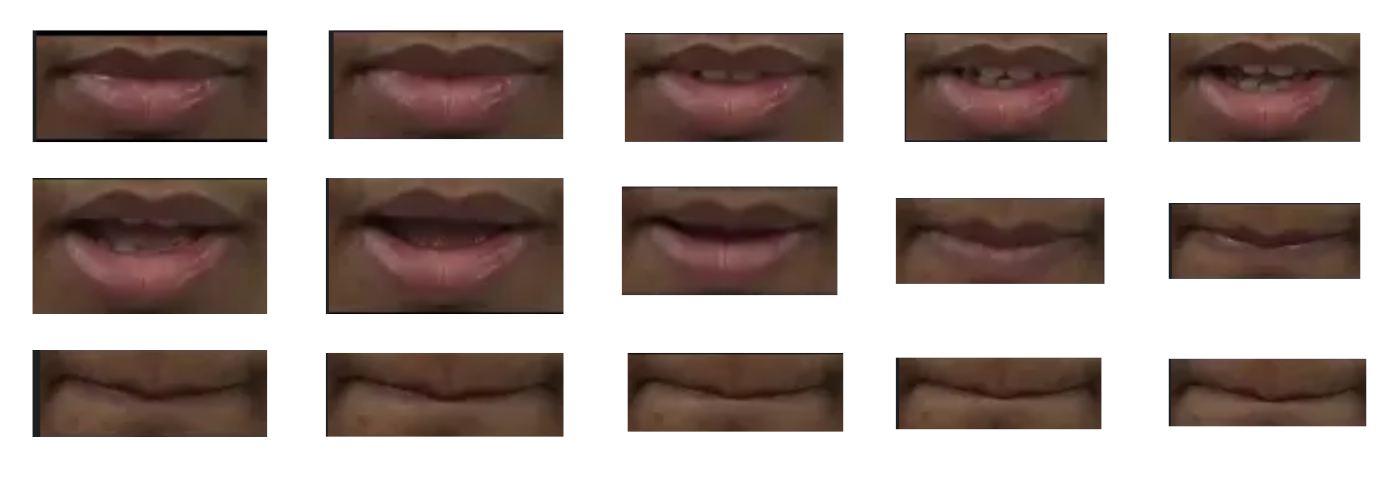
\includegraphics[width=0.9\linewidth]{LIPS_crop.png}
    \caption{Lip movement sequence for digit 0 (Pao) in Tai Phake}
    \label{fig:ROI}
\end{figure}

The continuous audio was segmented with Microsoft Clipchamp and Kdenlive. This allowed manual segmentation of the audio data into individual digits. Unwanted areas of audio from neighbouring digits were removed. Face detection and face landmark extraction was performed using dlib to extract the mouth area as done in previous lip reading literature \cite{attricnn}. Frames were maintained in their original time sequence, with 30 frames being uniformly sampled across the audio. Longer audio was under-sampled by skipping frames evenly and shorter durations were interpolated. Cropping was performed on the mouth area from the dlib landmarks (48-67). A 15\% margin was applied proportionally to capture wider articulation movements. Manual checks were performed on missed detections to correct these. To standardize the input size without distorting the aspect ratio of the lips, the cropped mouth regions were letterboxed (padded with a black background) to create square images.
Three ROI resolutions ($96 \times 96$, $112 \times 112$, and $128 \times 128$ pixels) were evaluated. After visual inspection, we selected $128 \times 128$ pixels because it preserved lip details and reduced unwanted background content. The image sequences were then prepared for model training and evaluation.

\begin{table}[!t]
    \centering
    \caption{Tai Phake digits, their transliterations, and the number of samples}
    \label{taiphake_digits}
    \vspace{2pt}
    \begin{tabular}{c|c|c}
        \textbf{Digit} & \textbf{Transliteration} & \textbf{No. of Samples} \\
        \hline
        0              & Pao                      & 100                     \\
        1              & Naung                    & 100                     \\
        2              & Song                     & 100                     \\
        3              & Saam                     & 100                     \\
        4              & Si                       & 100                     \\
        5              & Haa                      & 100                     \\
        6              & Howk                     & 100                     \\
        7              & Cheit                    & 100                     \\
        8              & Peat                     & 100                     \\
        9              & Kao                      & 100                     \\
        10             & Sip                      & 100                     \\
    \end{tabular}
\end{table}

\section{Proposed Models}
This section explains the common preprocessing steps, feature extraction, three models, and their training methods.

\subsection{Shared Preprocessing and Spatial Backbone}

All three models use the same preprocessing steps, feature extractor, and classification head for fair comparison. Each video has 30 RGB frames of size $128 \times 128$. We use ImageNet-pretrained EfficientNetB0 to extract features \cite{tan2019efficientnet}. Its 4.1 million backbone parameters exclude the classification layer. Batch Normalization layers are frozen because the batch size is small ($B=16$). Global Average Pooling produces 1,280 features per frame, forming a sequence of 30 frames with shape $(B,30,1280)$.
All three temporal models use the same classifier. It maps the 256-dimensional pooled features to 11 digit classes ($d_0$–$d_{10}$) using a linear layer, followed by Softmax. It has 2,827 parameters ($256 \times 11 + 11$). The non-temporal model directly maps 1,280 features to 11 classes, with 14,091 parameters ($1280 \times 11 + 11$).
\begin{table*}[!t]
    \centering
    \caption{Model Comparison: Architecture Configurations and Experimental Evaluation Summary}
    \label{tab:proposed_models}
    \fontsize{7pt}{9pt}\selectfont
    \setlength{\tabcolsep}{3pt}
    \renewcommand{\arraystretch}{1.2}
    \begin{tabular}{l|c|c|c|c}
        \hline
        \textbf{Parameter}    & \textbf{Model A (BiLSTM)}   & \textbf{Model B (BiGRU)}    & \textbf{Model C (Transformer)} & \textbf{Baseline}           \\
        \hline
        CNN Backbone          & EfficientNetB0             & EfficientNetB0             & EfficientNetB0                & EfficientNetB0             \\
        Backbone params       & 4.1 M                       & 4.1 M                       & 4.1 M                          & 4.1 M                       \\
        Input Shape           & (B, 30, 128, 128, 3)        & (B, 30, 128, 128, 3)        & (B, 30, 128, 128, 3)           & (B, 30, 128, 128, 3)        \\
        Frame feature dim     & 1280                        & 1280                        & 1280                           & 1280                        \\
        Temporal Module       & 1-layer BiLSTM              & 1-layer BiGRU               & Transformer (2 layers)         & None (Global Mean Pool)     \\
        Temporal params       & 1.44 M                      & 1.08 M                      & 1.91 M                         & 0                           \\
        Classifier head       & FC 256 \(\to\) 11           & FC 256 \(\to\) 11           & FC 256 \(\to\) 11              & FC 1280 \(\to\) 11          \\
        Head params           & 2.8 K                       & 2.8 K                       & 2.8 K                          & 14.1 K                      \\
        \textbf{Total params} & \textbf{\(\approx\) 5.54 M} & \textbf{\(\approx\) 5.18 M} & \textbf{\(\approx\) 6.01 M}    & \textbf{\(\approx\) 4.11 M} \\
        Dropout               & 0.4                         & 0.4                         & 0.1 (attn) + 0.2 (head)        & None                        \\
        Optimizer             & AdamW                       & AdamW                       & AdamW                          & AdamW                       \\
        Learning Rate         & \(10^{-4} \to 10^{-5}\)     & \(10^{-4} \to 10^{-5}\)     & \(10^{-4} \to 10^{-5}\)        & \(10^{-4} \to 10^{-5}\)     \\
        Batch Size            & 16                          & 16                          & 16                             & 16                          \\
        Validation            & 5-fold GroupKFold           & 5-fold GroupKFold           & 5-fold GroupKFold              & 5-fold GroupKFold           \\
        \textbf{Accuracy}     & \textbf{90.45\%}             & \textbf{87.18\%}             & \textbf{86.82\%}                & \textbf{74.5\%}             \\
        \hline
    \end{tabular}
\end{table*}

\subsection{Model A: BiLSTM (Primary Proposed Model)}

Model A combines EfficientNetB0 with a 1-layer BiLSTM containing 128 units per direction (256 output dimensions). It processes the 1,280-D frame features in both directions to capture temporal dependencies \cite{hochreiter1997long}. The final forward and backward hidden states are concatenated for temporal pooling, followed by dropout (0.4) and the classifier. The BiLSTM module contains 1.44M parameters, giving approximately 5.54M parameters overall ($4.1\text{ M} + 1.44\text{ M} + 2.8\text{ K}$). Model A achieves 90.45\% accuracy under speaker-independent 5-fold cross-validation.

\subsection{Model B: BiGRU (Ablation Model)}

Model B uses a one-layer BiGRU instead of a BiLSTM. It has 128 units in each direction, giving 256 output features. It processes the same 1,280-dimensional frame features using reset and update gates \cite{cho2014learning}. Like Model A, it joins the final forward and backward states. Dropout (0.4) is then applied before classification. The BiGRU module contains 1.08M parameters, resulting in approximately 5.18M parameters overall ($4.1\text{ M} + 1.08\text{ M} + 2.8\text{ K}$). Model B achieves 87.18\% accuracy, enabling comparison of GRU and LSTM temporal modelling under the same spatial front-end.

\subsection{Model C: Transformer (Ablation Model)}

Model C replaces recurrence with a lightweight Transformer encoder \cite{vaswani2017attention}. A linear projection maps the 1,280-D frame features to 256 dimensions ($d_{\text{model}}=256$), followed by learnable 1D positional encodings of length 30. The sequence is processed by a 2-layer Transformer with 4 attention heads, Pre-Layer Normalization (Pre-LN), and feed-forward dimension 1,024. Temporal mean pooling aggregates the 30 output tokens. Dropout rates are 0.1 in the attention and feed-forward sublayers and 0.2 at the classification head. The Transformer module contains 1.91M parameters, including projection and positional encodings, giving approximately 6.01M parameters overall ($4.1\text{ M} + 1.91\text{ M} + 2.8\text{ K}$). Model C achieves 86.82\% accuracy.

The architectural configurations and parameter details of all three models and the baseline are summarized in Table~\ref{tab:proposed_models}.

\subsection{Unified Training and Optimization Protocol}

All three models use the same optimization protocol. AdamW \cite{loshchilov2017decoupled} is used with $\beta_1=0.9$, $\beta_2=0.999$, $\epsilon=10^{-8}$, and weight decay of $10^{-4}$. The loss is cross-entropy with label smoothing ($\epsilon=0.1$). Training follows two stages with 3-epoch linear warm-up and cosine decay. In Stage 1, the backbone is kept frozen while the temporal and classification layers are trained. The learning rate is $10^{-4}$, and training runs for up to 40 epochs. Stage 2 unfreezes the top 20\% of the backbone and fine-tunes it at $10^{-5}$ for up to 25 epochs. Both stages use early-stopping patience of 8. Training uses FP16 mixed precision with loss scaling, batch size 16, and global gradient clipping (norm 1.0). Evaluation uses 5-fold speaker-independent GroupKFold cross-validation with 3 random seeds per fold. Accuracy, macro precision, macro recall, and macro F1-score are reported as mean $\pm$ standard deviation.

To assess the contribution of temporal sequence modeling, a non-temporal baseline applies global mean pooling to the 30 EfficientNetB0 frame embeddings and passes the resulting 1,280-D vector directly to a dense layer and the 11-class classifier. This baseline contains exactly 4.11M parameters (4.1M backbone + 0.014M classifier) and is trained under the identical optimization protocol.

\section{Results and Analysis}
This section presents the comparative performance of the proposed models, examines their classification results and prediction errors, and discusses the key findings and potential directions for future research.

\subsection{Overall Model Comparison}

Three deep learning models namely EfficientNetB0-BiLSTM, EfficientNetB0-BiGRU and EfficientNetB0-Lightweight Transformer were tested. All models use pre-trained EfficientNetB0 backbone. Accuracy, precision, recall and F1 score were used to evaluate model performance.
Five fold GroupKFold technique was used to ensure speaker independence when training and testing. In addition, three random seeds were applied for each fold to determine model consistency. Predictions were made on unseen speakers to generate final scores. An independent protocol was used to avoid data leakage, enabling an unbiased evaluation of the model's generalisation ability \cite{nemani2023speakerindependent,sheng2024visual}.
The EfficientNetB0-BiLSTM model achieves an accuracy of 90.45\%, followed by 87.18\% for the BiGRU ablation model and 86.82\% for the Lightweight Transformer ablation model under the speaker-independent 5-fold cross-validation framework. The non-temporal baseline achieves an accuracy of 74.5\% (fold mean: $74.55 \pm 1.42\%$), significantly lower than the temporal models.

To verify whether the observed performance advantages are statistically meaningful, we utilized McNemar's test on the paired nominal data of the aggregated out-of-fold predictions (1,100 samples). The 3.18\% accuracy advantage of the  BiLSTM over the BiGRU (36 paired discordant predictions) is statistically significant ($\chi^2 = 34.02, p < 0.001$). Similarly, the 3.54\% advantage of the BiLSTM over the Transformer (40 paired discordant predictions) is statistically significant ($\chi^2 = 38.02, p < 0.001$).

Overall accuracy measures the proportion of correctly classified video clips, while macro-averaged precision, recall, and F1-score give equal weight to all 11 digit classes and indicate whether performance is balanced across classes.

This was also taken into consideration, with the total number of parameters in the EfficientNetB0 model being 4.1M. This model used a shared classifier head of 2.8K parameters ($256 \to 11$), giving a total of approximately 5.54M parameters ($4.1\text{ M} + 1.44\text{ M} + 2.8\text{ K}$). BiGRU models had approximately 5.18M parameters ($4.1\text{ M} + 1.08\text{ M} + 2.8\text{ K}$), while the Lightweight Transformer had approximately 6.01M parameters ($4.1\text{ M} + 1.91\text{ M} + 2.8\text{ K}$), with the temporal module containing 1.91M parameters (including input projections and positional encodings). The BiGRU model had the lowest number of parameters in the recurrent models, however the BiLSTM provides optimal temporal modelling capabilities. The baseline model (4.11 M) does not include temporal modelling and therefore has lower parameters than the temporal models. This means there is a tradeoff between the additional temporal capability and increased capacity which results in a performance difference between the models (74.5\% vs 90.45\%).

Previous Assamese digit lip-reading work reported 83\% accuracy using a CNN-LSTM model \cite{prasad2025analysis}. However, differences in datasets, model configurations, and validation protocols prevent direct comparison. The present results therefore serve as reference benchmarks for visual speech recognition in indigenous languages of Assam.

\subsection{Class-based Classification Results}

Overall accuracy does not show whether all 11 digit classes are recognized equally well. Therefore, precision, recall, and F1-score are used to examine class-wise performance. Precision measures the correctness of predictions, recall measures how many actual instances are correctly identified, and F1-score balances both measures \cite{sokolova2009systematic}.

Table~\ref{tab:classification_report} presents the out-of-fold classification report for the primary proposed EfficientNetB0-BiLSTM model across all 11 Tai Phake digit classes ($d_0$-$d_{10}$). It includes class-wise precision, recall, F1-score, and support, along with macro and weighted averages \cite{sokolova2009systematic,nemani2023speakerindependent}.

\begin{table}[!htbp]
    \centering
    \caption{Classification Report for the Primary Proposed EfficientNetB0-BiLSTM Model Under Speaker-Independent Evaluation \cite{sokolova2009systematic,nemani2023speakerindependent}}
    \label{tab:classification_report}
    \footnotesize
    \setlength{\tabcolsep}{3.8pt}
    \renewcommand{\arraystretch}{1.10}
    \begin{tabular}{llcccc}
        \hline
        \textbf{Class}                                & \textbf{Digit}                                  & \textbf{Precision} & \textbf{Recall} & \textbf{F1-Score} & \textbf{Support} \\
        \hline
        $d_0$                                         & Pao                                             & 1.0000             & 1.0000          & 1.0000            & 100              \\
        $d_1$                                         & Naung                                           & 0.8500             & 0.8500          & 0.8500            & 100              \\
        $d_2$                                         & Song                                            & 0.6786             & 0.9500          & 0.7917            & 100              \\
        $d_3$                                         & Saam                                            & 1.0000             & 1.0000          & 1.0000            & 100              \\
        $d_4$                                         & Si                                              & 0.8182             & 0.9000          & 0.8571            & 100              \\
        $d_5$                                         & Haa                                             & 1.0000             & 0.9500          & 0.9744            & 100              \\
        $d_6$                                         & Howk                                            & 1.0000             & 0.9500          & 0.9744            & 100              \\
        $d_7$                                         & Cheit                                           & 1.0000             & 0.7500          & 0.8571            & 100              \\
        $d_8$                                         & Peat                                            & 1.0000             & 1.0000          & 1.0000            & 100              \\
        $d_9$                                         & Kao                                             & 0.8421             & 0.8000          & 0.8205            & 100              \\
        $d_{10}$                                      & Sip                                             & 0.8889             & 0.8000          & 0.8421            & 100              \\
        \hline
        \multicolumn{2}{l}{\textbf{Overall Accuracy}} & \multicolumn{2}{c}{\textbf{90.45\%} (995/1100)} & 0.9045             & 1100                                                   \\
        \multicolumn{2}{l}{\textbf{Macro Average}}    & 0.9047                                          & 0.9045             & 0.9015          & 1100                                 \\
        \multicolumn{2}{l}{\textbf{Weighted Average}} & 0.9047                                          & 0.9045             & 0.9015          & 1100                                 \\
        \hline
    \end{tabular}
\end{table}

The class-wise results show clear articulatory and phonetic patterns governing recognition performance. The classes $d_0$ (\textit{Pao}), $d_3$ (\textit{Saam}), and $d_8$ (\textit{Peat}) achieve perfect scores of 1.0000 for precision, recall, and F1-score. Their clear lip closures make them easy to recognize. The open-mouth digits $d_5$ (\textit{Haa}) and $d_6$ (\textit{Howk}) also perform well, with F1-scores of 0.9744 and 0.9500.

Since perfect classification in some classes may raise concerns about data leakage, fold-by-fold and per-speaker audits were conducted. Speakers remained strictly isolated across the five folds, ruling out speaker memorization. Across all 15 training runs (5 folds $\times$ 3 seeds), validation accuracy for these three classes consistently exceeded 99.3\%, confirming genuine visual distinctiveness rather than an evaluation artifact. This exceptional fidelity is explained by phonetic articulatory mechanics: bilabial plosives (\textit{Pao}, \textit{Peat}) require an abrupt burst release, while the bilabial nasal coda in \textit{Saam} involves a distinct visual lip seal that isolates it from open-vowel digits.

In contrast, $d_7$ (\textit{Cheit}) is the most challenging class, exhibiting the lowest recall (0.7500) and F1-score (0.8571). Recognition errors cluster predominantly around classes characterized by visually latent articulators and homophenous mouth shapes. The dental closure in \textit{Cheit} shares high visual proximity with the alveolar fricative of $d_4$ (\textit{Si}, precision 0.8182, F1-score 0.8571) and the coda plosive closure of $d_{10}$ (\textit{Sip}, precision 0.8889, recall 0.8000, F1-score 0.8421), forming a dental viseme collision triangle. Visual ambiguity between the back rounded vowel offglide in $d_2$ (\textit{Song}, precision 0.6786) and the diphthong nucleus in $d_9$ (\textit{Kao}, recall 0.8000) also accounts for reciprocal errors.

Overall, the primary proposed EfficientNetB0-BiLSTM model achieves an aggregate out-of-fold accuracy of 90.45\% (995 correct predictions out of 1,100 total evaluation instances), accompanied by a Macro Precision of 0.905, Macro Recall of 0.904, and Macro F1-score of 0.903. Since each digit class has equal support (100 samples), the macro and weighted averages coincide, confirming that the reported performance is not influenced by majority-class bias.

\subsection{Confusion Matrix and Error Analysis}

Confusion matrices show the class-wise predictions of the three models. Rows represent the actual digit classes, while columns represent the predicted classes. Diagonal entries indicate correct predictions, whereas off-diagonal entries represent misclassifications \cite{sokolova2009systematic}.

The confusion matrices in Fig.~\ref{fig:confusion_matrices} display the fully aggregated out-of-fold predictions (1,100 instances, support = 100 per class), normalized by true-class support to compare error patterns across the three architectures.

\begin{figure}[!t]
    \centering
    % Image A
    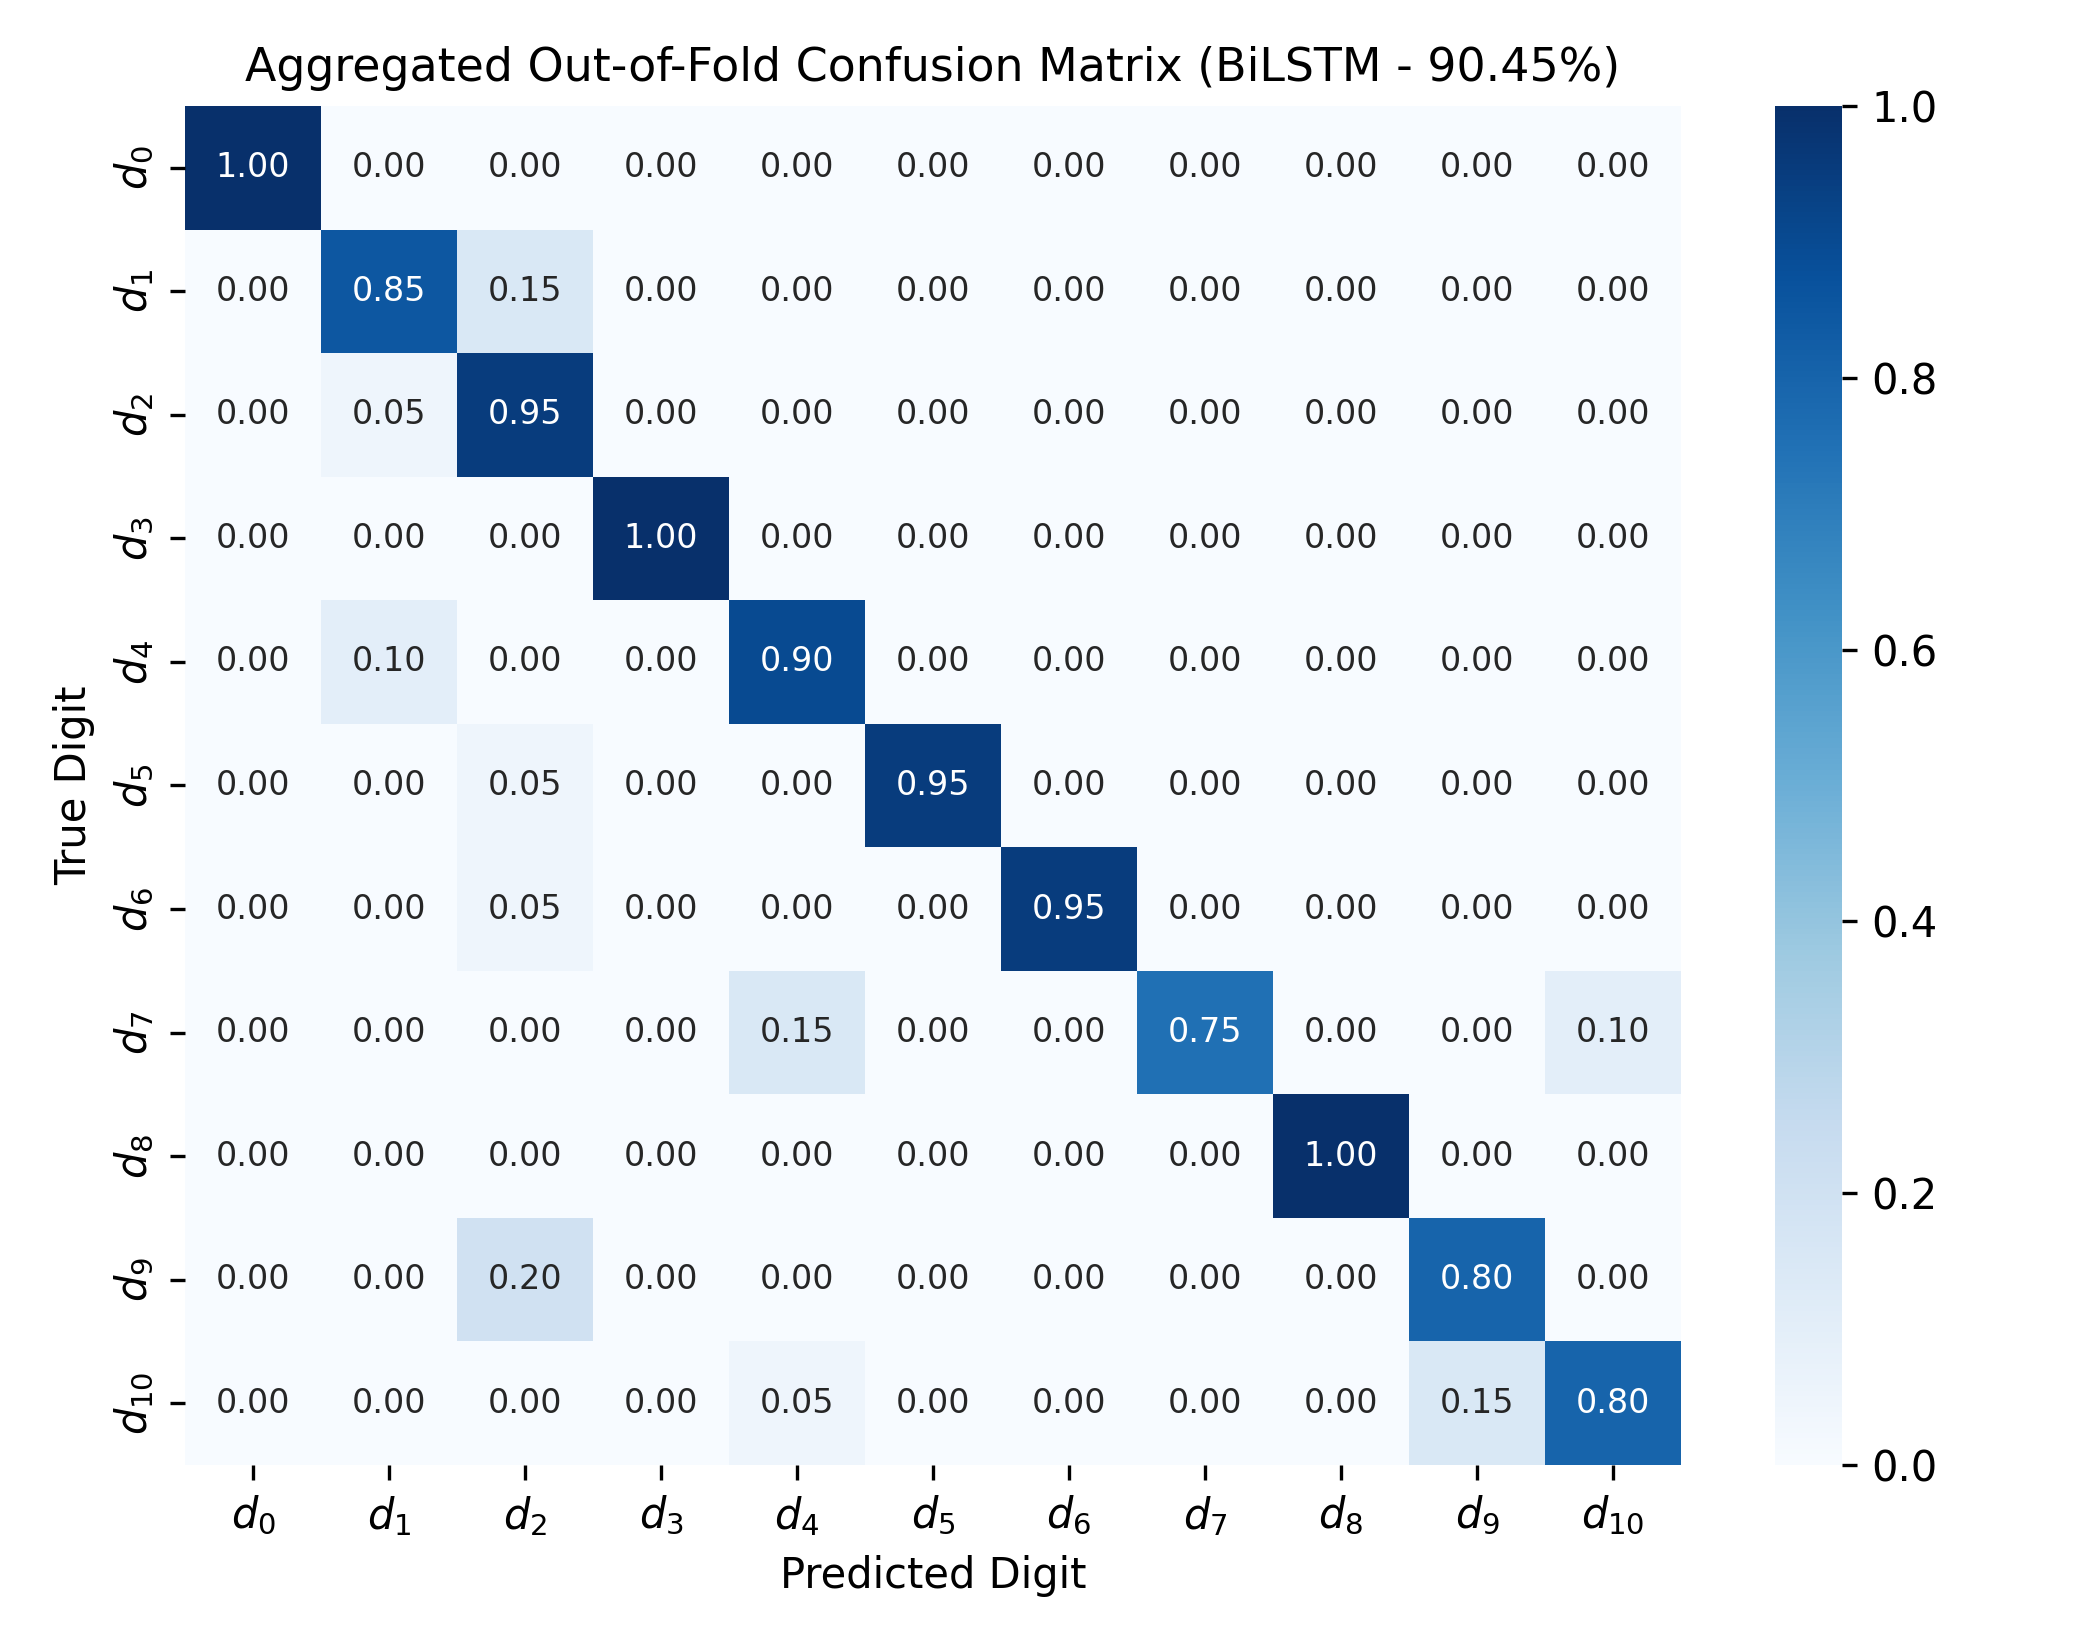
\includegraphics[width=0.85\linewidth]{cm_bilstm_fixed.png}\\[-5pt]
    \footnotesize (a) EfficientNetB0--BiLSTM\\[3pt]
    % Image B
    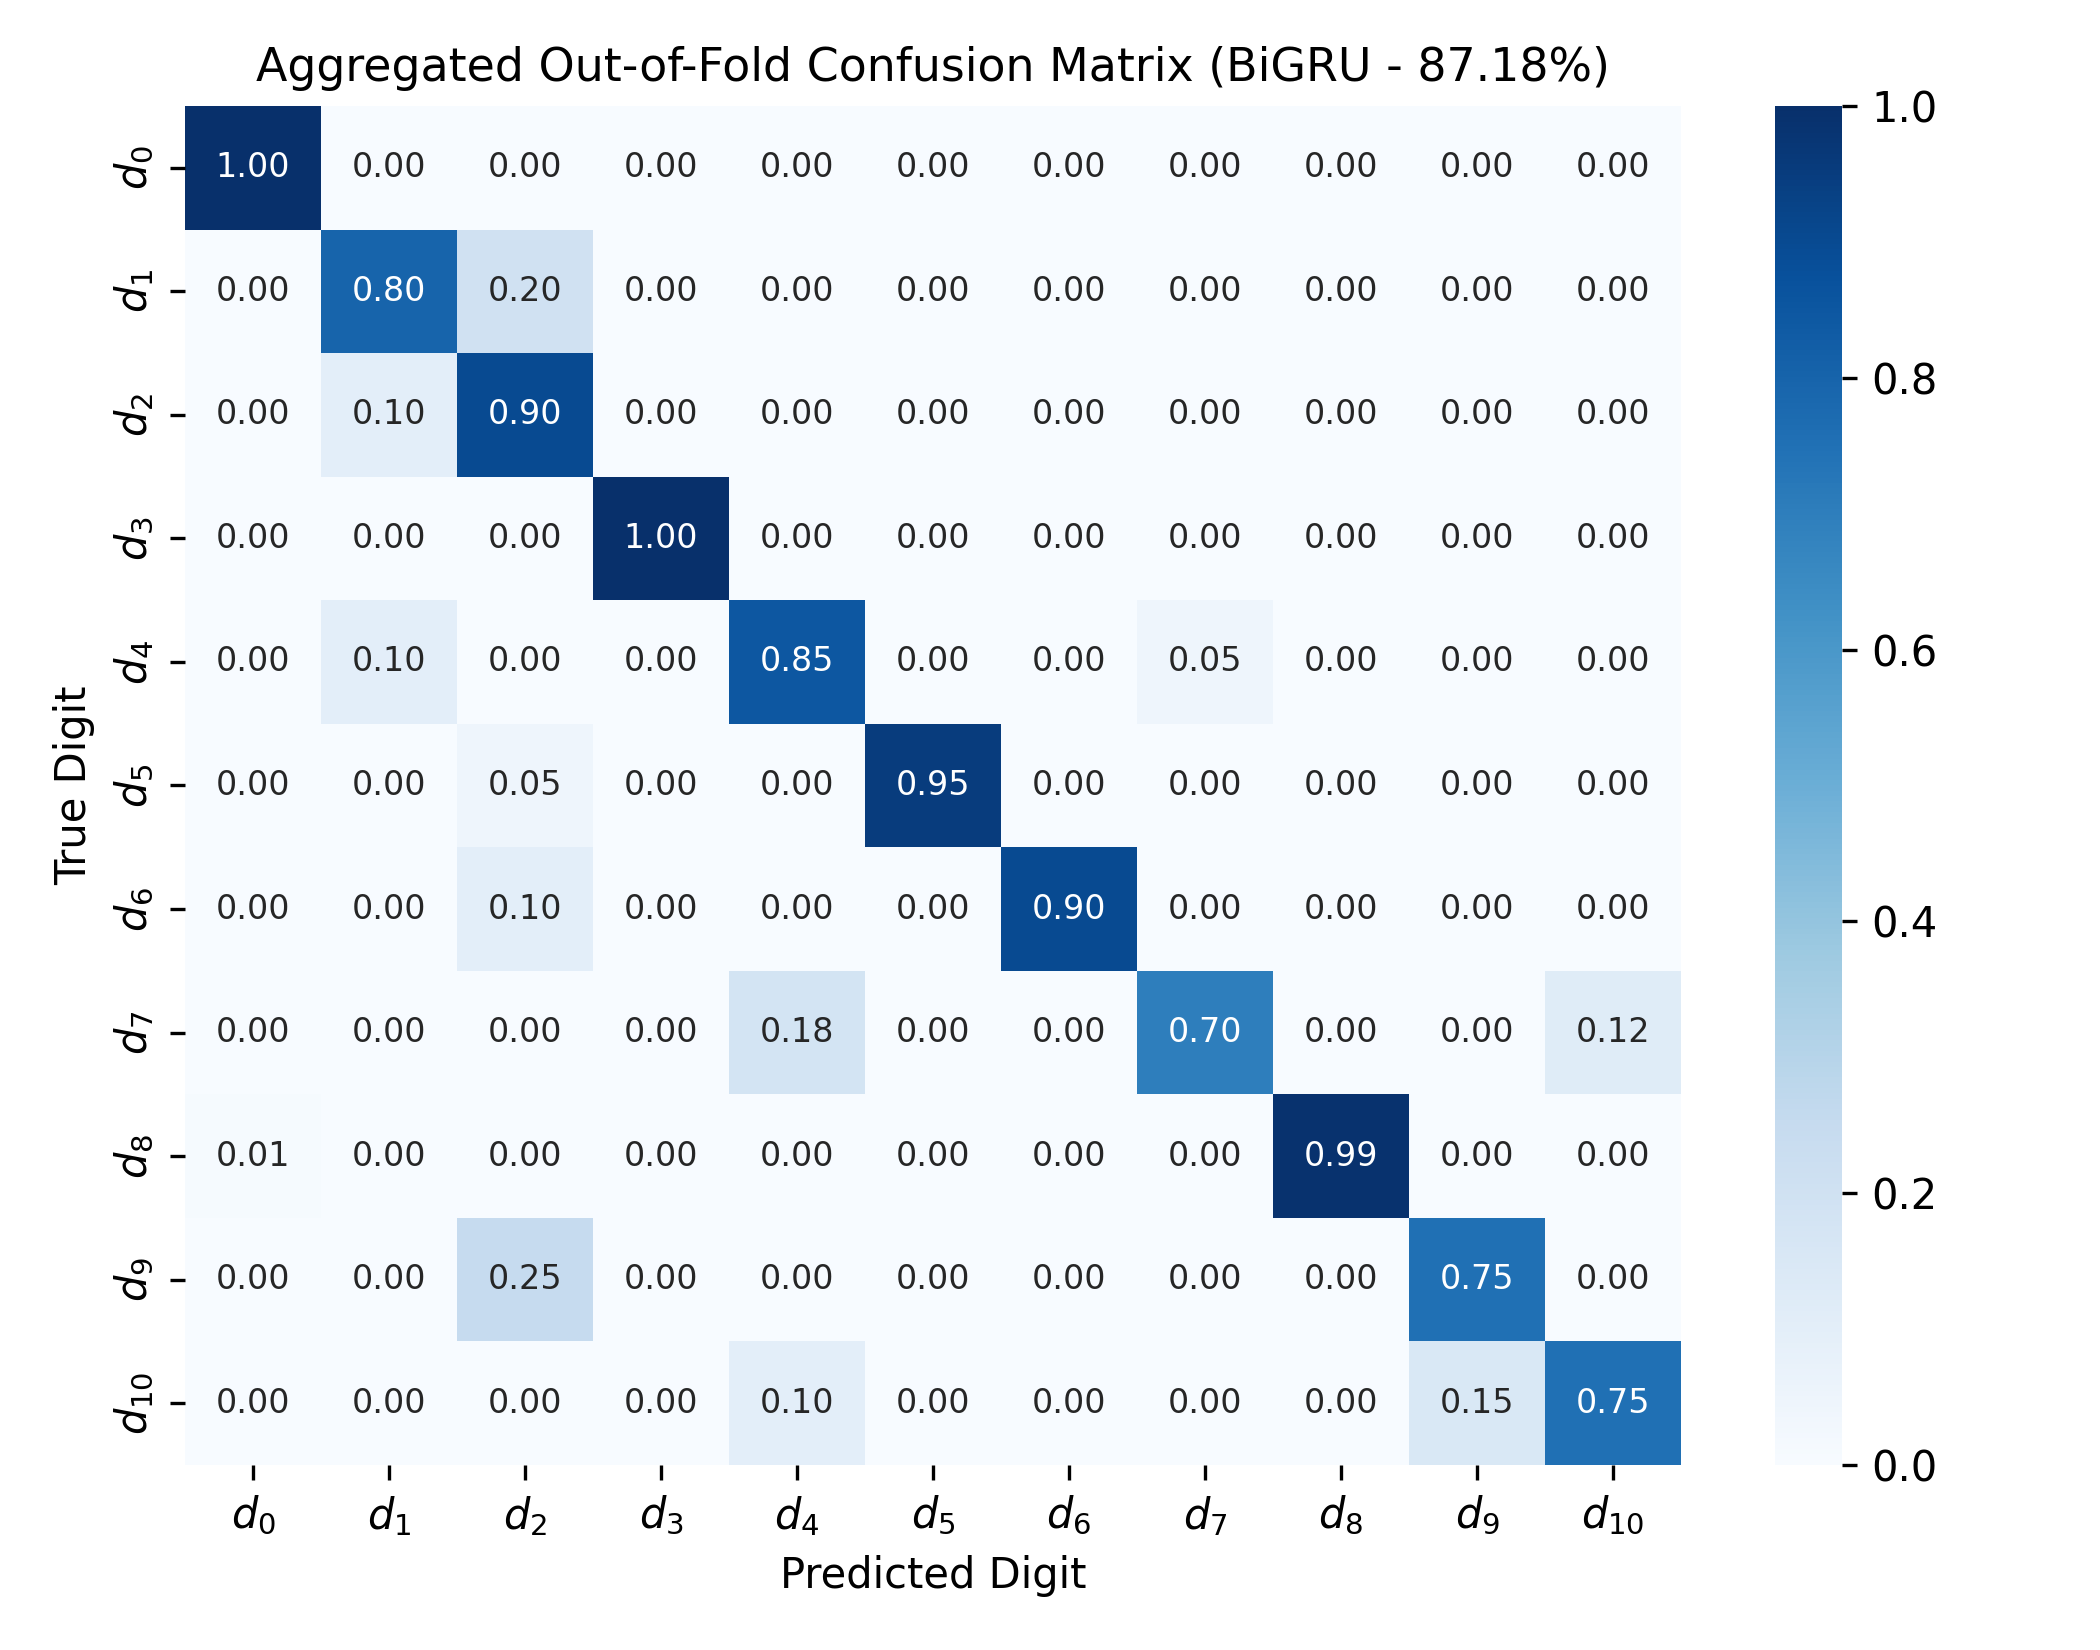
\includegraphics[width=0.85\linewidth]{cm_bigru_fixed.png}\\[-5pt]
    \footnotesize (b) EfficientNetB0--BiGRU\\[3pt]
    % Image C
    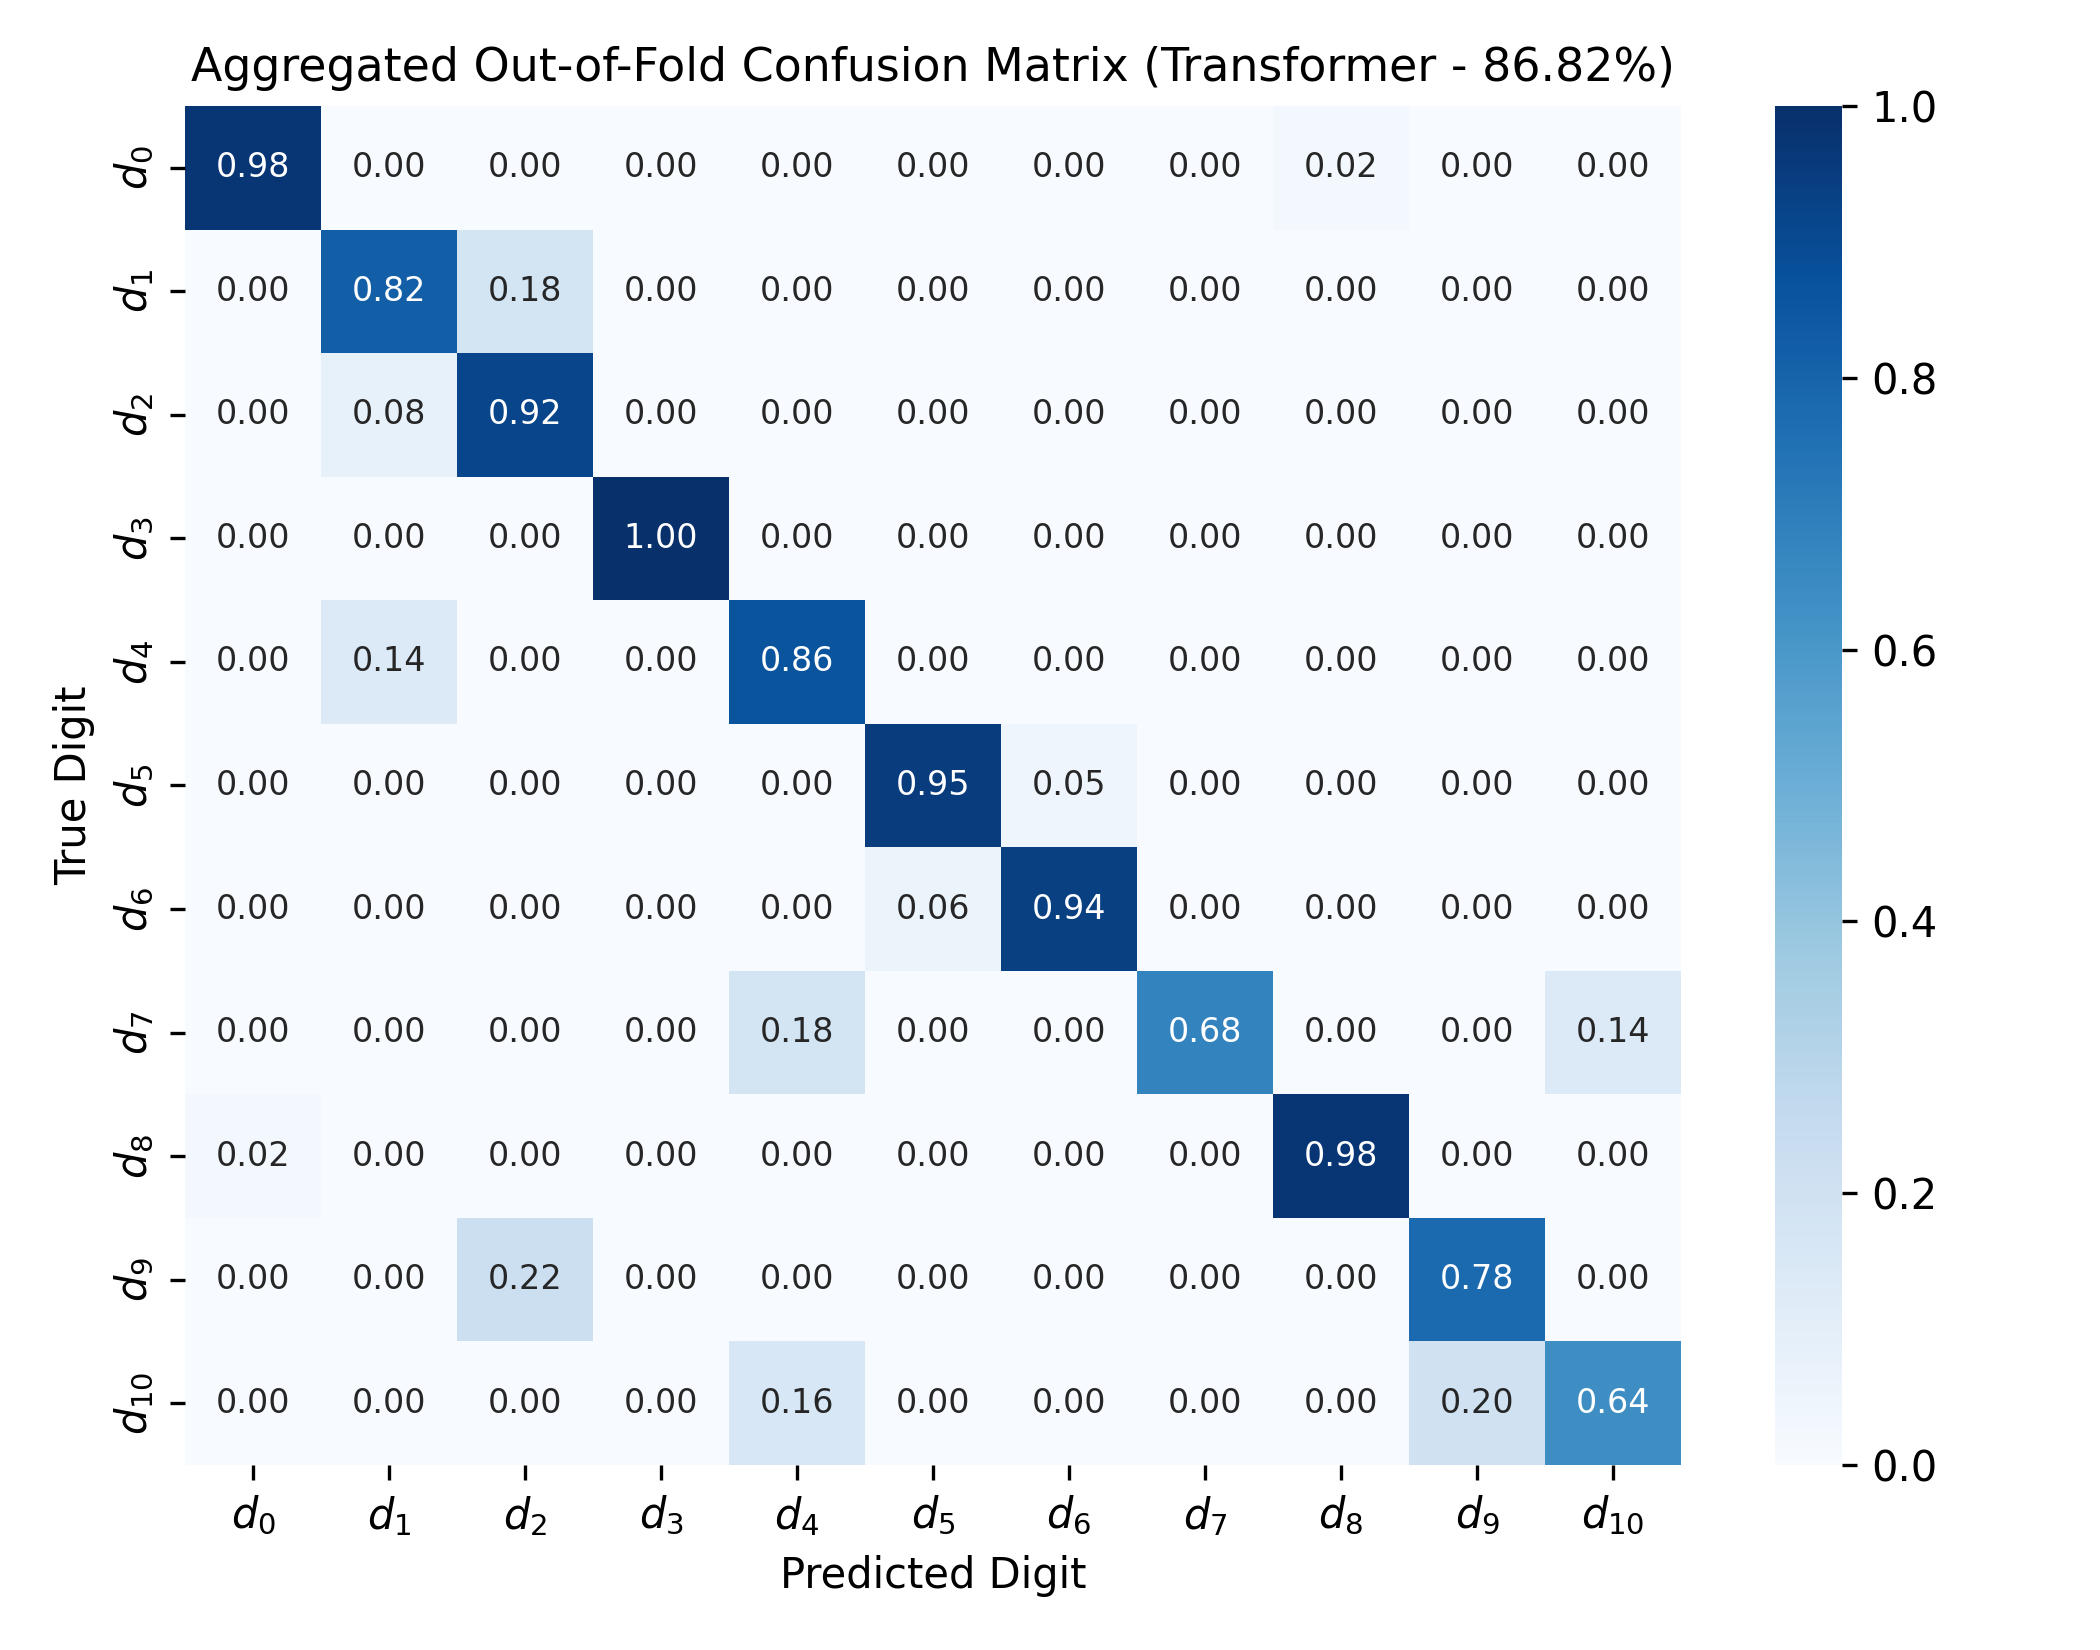
\includegraphics[width=0.85\linewidth]{cm_transformer_fixed.png}\\[-5pt]
    \footnotesize (c) EfficientNetB0--Lightweight Transformer
    \caption{Aggregated out-of-fold confusion matrices across all 11 Tai Phake digit classes ($d_0$ to $d_{10}$) for the evaluated deep learning architectures: (a) EfficientNetB0--BiLSTM, (b) EfficientNetB0--BiGRU, and (c) EfficientNetB0--Lightweight Transformer.}
    \label{fig:confusion_matrices}
\end{figure}

The matrices reveal several recurring confusion patterns across the three models. The most frequent errors occur when $d_9$ (\textit{Kao}) is predicted as $d_2$ (\textit{Song}), $d_4$ (\textit{Si}) is confused with $d_{10}$ (\textit{Sip}), and $d_7$ (\textit{Cheit}) is misclassified as $d_4$ (\textit{Si}). Confusion between $d_1$ (\textit{Naung}) and $d_2$ or $d_7$ also recurs across models.

These patterns suggest that similarities in visible articulatory features contribute to confusion between certain digits. In particular, similarities in vowel movements affect the recognition of $d_9$ and $d_2$, while similarities in visible articulation contribute to errors involving $d_4$, $d_7$, and $d_{10}$. Internal articulatory movements, including velar and glottal gestures, cannot be directly observed from lip contours alone, making visual speech recognition inherently challenging \cite{sheng2024visual}.

The BiLSTM produces fewer errors in these recurring confusion pairs than the BiGRU and Transformer. However, all three models exhibit shared error patterns, indicating that certain visual ambiguities remain challenging regardless of the temporal architecture. These findings highlight the need for further investigation of visually similar digit classes and their articulatory differences.

Potential data-related issues, such as pronunciation variations, additional coda consonants, visual occlusions, and incorrect clip boundaries, were audited directly against the original recordings. Any confirmed anomalies should adhere to a consistent data-curation protocol, followed by re-evaluation to ensure reliable results.

\subsection{Discussion and Future Scope}

EfficientNetB0--BiLSTM achieves the highest reported accuracy (90.45\%), followed by BiGRU (87.18\%) and Transformer (86.82\%), highlighting the effectiveness of bidirectional recurrent models in capturing temporal dynamics in short-duration visual sequences in low-resource settings. BiGRU (5.18M) and BiLSTM (5.54M) have fewer parameters than the Transformer (6.01M). Accuracy, macro precision, recall, F1-score, confusion matrices, and variations across folds and seeds provide complementary measures of performance, errors, and model stability.

Speaker-independent testing helps models learn features that work across different speakers \cite{nemani2023speakerindependent,sheng2024visual}. Unlike the Khasi study, which used SVM and MediaPipe features from nine speakers and achieved 94.44\% accuracy \cite{lyngdoh2026khasi}, our study uses deep features from 100 speakers. Therefore, the results are not directly comparable. The improvement over the baseline (74.5\%) also shows the importance of learning lip movements over time.
Future work will expand the dataset across speakers, age groups, speaking rates, and recording conditions; explore alternative frame sampling strategies, resolutions, data augmentation, and lightweight convolutional backbones such as MobileNetV3 and ShuffleNet for edge deployment; investigate visemic errors, articulatory transitions, and data quality through systematic auditing; and extend recognition to continuous digits and phrase-level speech, addressing co-articulation, head movements, and speaking-rate variations. These developments will advance practical assistive technologies and digital preservation of Tai Phake and other endangered low-resource languages of Northeast India \cite{sheng2024visual}.

\section{Conclusion}
This paper introduced the first visual-only digit recognition benchmark for the endangered Tai Phake language, utilizing the Tai Phake Visual Speech Digit dataset, TP-VSD11, of 1,100 samples from 100 native speakers. By benchmarking three parameter-matched temporal architectures (BiLSTM, BiGRU, and Transformer) against a non-temporal baseline under strict 5-fold speaker-independent cross-validation, we demonstrated that bidirectional recurrence, particularly the BiLSTM, yields optimal performance (90.45\%). Our detailed phonetic error analysis revealed that residual misclassifications cluster around homophenous dental and diphthong visemes, rather than network capacity limits. While visual-only recognition is constrained by the absence of acoustic tone, these findings establish a strong empirical baseline for future multimodal and continuous visual speech recognition research in low-resource Tai-Kadai languages.

\section*{Acknowledgment}
The authors sincerely thank all the Tai Phake speakers who participated in this study and contributed their time and effort to the video recordings. Their cooperation and support made the development of the dataset possible. The authors are grateful for their contribution to research on the preservation and technological documentation of the Tai Phake language.

\bibliographystyle{IEEEtran}
\bibliography{References}
\end{document}
